\documentclass[12pt]{article}
 
\usepackage[margin=1in]{geometry}
\usepackage{amsmath,amsthm,amssymb}
\usepackage{fancyhdr}
\usepackage{hyperref}
\pagestyle{fancy}
\usepackage{graphicx}
\newcommand{\N}{\mathbb{N}}
\newcommand{\R}{\mathbb{R}}
\newcommand{\Z}{\mathbb{Z}}
\newcommand{\Q}{\mathbb{Q}}
 
\newenvironment{theorem}[2][Theorem]{\begin{trivlist}
\item[\hskip \labelsep {\bfseries #1}\hskip \labelsep {\bfseries #2.}]}{\end{trivlist}}
\newenvironment{lemma}[2][Lemma]{\begin{trivlist}
\item[\hskip \labelsep {\bfseries #1}\hskip \labelsep {\bfseries #2.}]}{\end{trivlist}}
\newenvironment{exercise}[2][Exercise]{\begin{trivlist}
\item[\hskip \labelsep {\bfseries #1}\hskip \labelsep {\bfseries #2.}]}{\end{trivlist}}
\newenvironment{problem}[2][Problem]{\begin{trivlist}
\item[\hskip \labelsep {\bfseries #1}\hskip \labelsep {\bfseries #2.}]}{\end{trivlist}}
\newenvironment{question}[2][Question]{\begin{trivlist}
\item[\hskip \labelsep {\bfseries #1}\hskip \labelsep {\bfseries #2.}]}{\end{trivlist}}
\newenvironment{corollary}[2][Corollary]{\begin{trivlist}
\item[\hskip \labelsep {\bfseries #1}\hskip \labelsep {\bfseries #2.}]}{\end{trivlist}}
 
\begin{document}
 
\title{Lab 3: File Servers, Traffic Generators, and Monitoring}
\author{Duc Viet Le\\
 CS536}
 
\maketitle
 
\begin{problem}{1} \ \\
For this problem, I use an audio file (i.e.) with file size of 3183357 bytes ($\approx 3.1$ MB). I use both check sum and Linux \texttt{diff} to check for the authenticity of the downloaded files. With TCP, we did not have any corrupted files. 
\\
Below are the results of time and through put for different package sizes:
\begin{center}
	\begin{tabular}{|c|c|c|}
	\hline 
	Package size & Time & Reliable Through Put \\ \hline
	1 byte & 5265 ms & 4,836,939 bps \\ \hline
	10 bytes & 590 ms & 43,152,693 bps \\ \hline
	50 bytes & 276 ms & 92,095,696 bps \\ \hline
	500 bytes & 274 ms & 92,382,231 bps \\ \hline
	1000 bytes & 273 ms & 93,115,342 bps \\ \hline
	1500 bytes & 272 ms & 92,695,123 bps \\ \hline
	2500 bytes & 273 ms & 93,255,654 bps \\ \hline
	10000 bytes & 275 ms & 92,895,832 bps \\ \hline
	\end{tabular}
\end{center}
Below is plotted graph of the data: \\
\begin{figure}
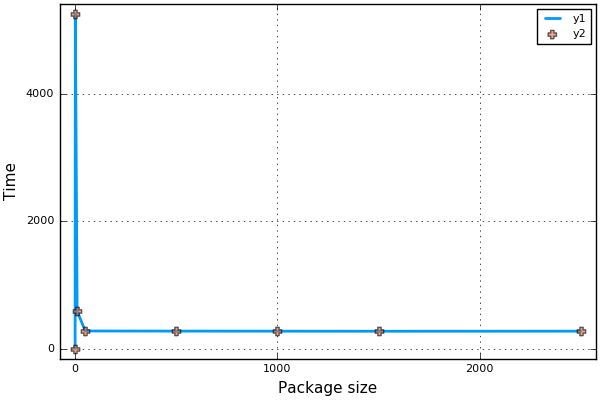
\includegraphics[scale = .6]{1.png}
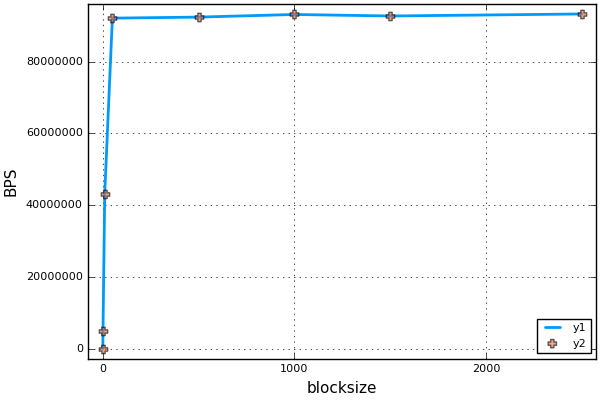
\includegraphics[scale = .6]{2.png} 
\end{figure}
\\
While the small package size may limit reliable through put, much bigger package size also does not have much impact on throughput. As the package size reach a certain value, the reliable throughput and transmission time did not change. Thus, to improve the server performance, I may choose package size to be power of two because it may be helpful for computers and kernels, not too big so that we can fit inside processor (i.e L2 cache) ... 
\end{problem}
\begin{problem}{2} \ \\
For payload-size = $1000$ bytes, packet-count = $1000$. We obtain the following result with different packet-spacing:\\
\texttt{Traffic\_rcv} was run at $sslab01$. \texttt{Traffic\_snd} was run at my home. 
\begin{center}
	\begin{tabular}{|c|c|c|c|c|c|c|}
	\hline 
	& \multicolumn{3}{|c|}{Sender} & \multicolumn{3}{|c|}{Receiver}\\ \hline
	Packet Spacing 		   & Time& BPS& PPS& Time &BPS& PPS\\ \hline
	50ms 		  		   & 50.136s &  167965 bps& 20 pps & 50.141 s &167679 bps&20 pps\\ \hline
	10ms 		  		   & 10.125s &  831171 bps& 99 pps & 10.126 s &830265 bps&99 pps\\ \hline
	1ms 		  		   & 1.128s &  7457984 bps& 886 pps & 1.127 s &7466294 bps& 887 pps\\ \hline
	.5ms 		  		   & .596s &  14119573 bps& 1678 pps & .599 s &14035791 bps&1667 pps\\ \hline
	.1ms 		  		   & .226s &  37289592 bps& 3923 pps & .223 s &37680936 bps&3916 pps\\ \hline
	\end{tabular}
\end{center}
Graph: \\
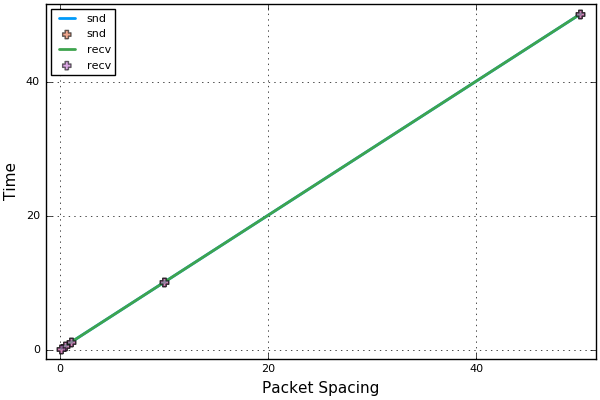
\includegraphics[scale=.6]{3.png}
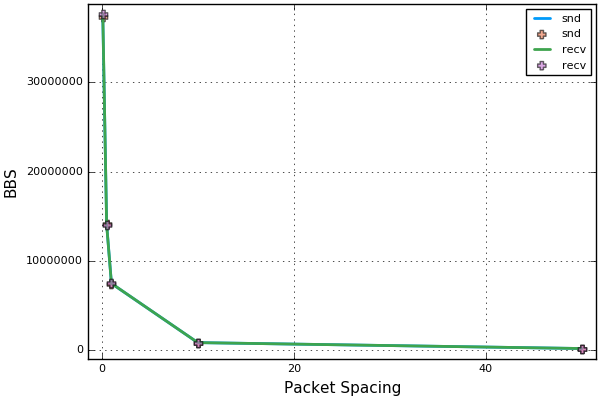
\includegraphics[scale=.6]{4.png}\\
\begin{center}
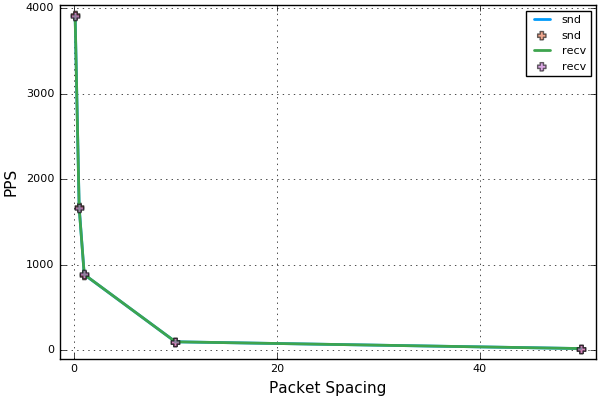
\includegraphics[scale=.6]{5.png}	
\end{center}
Yes, throughput numbers are approximately equal for both client and server. When package spacing reduces from 50ms to .1 ms, completion decreases, throughput increases, and pps increases. Yes, I think the observed result are consistent with what theoretically expected because by reducing the spacing time, we allow the receiver to process incoming datagram with faster rate. Hover, after reducing the time spacing to less than equal to $.1$ ms, I don't see any improvement in completion time, so I think the OS process reaches its limit to handle \texttt{recvfrom}.\\
For payload-size = $10000$ bytes, packet-spacing = $1$ ms. We obtain the following result with different packet-spacing:\\
\begin{center}
	\begin{tabular}{|c|c|c|c|c|c|c|}
	\hline 
	& \multicolumn{3}{|c|}{Sender} & \multicolumn{3}{|c|}{Receiver}\\ \hline
	Packet size 		   	   & Time& BPS& PPS& Time &BPS& PPS\\ \hline
	50 bytes 		  		   & 11.234s &  737458.188 bps& 886 pps & 11.282 s &727746 bps& 890 pps\\ \hline
	500 bytes 		  		   & 11.238s &  3929357 bps& 889 pps & 11.239 s & 3929083 bps & 889 pps\\ \hline
	1000 bytes 		  		   & 11.362s &  7407060 bps& 880 pps & 11.390 s &7388543 bps  & 877 pps\\ \hline
	2000 bytes 		  		   & 11.406s &  14398335 bps& 877 pps & 11.399 s &14399694 bps& 877 pps\\ \hline
	4000 bytes 		  		   & 11.388s &  28465396 bps& 878 pps & 11.388 s &28463406 bps& 878 pps\\ \hline
	8000 bytes 		  		   & 18.675s &  34492452 bps& 535 pps & 534.986 s &34461664 bps&534 pps\\ \hline
	\end{tabular}
\end{center}
Graphs:\\
\\
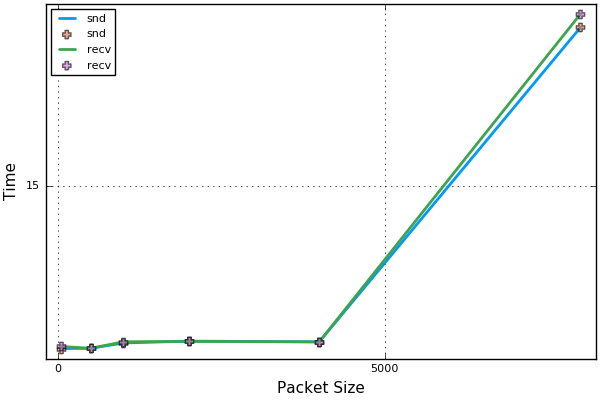
\includegraphics[scale=.6]{6.png}
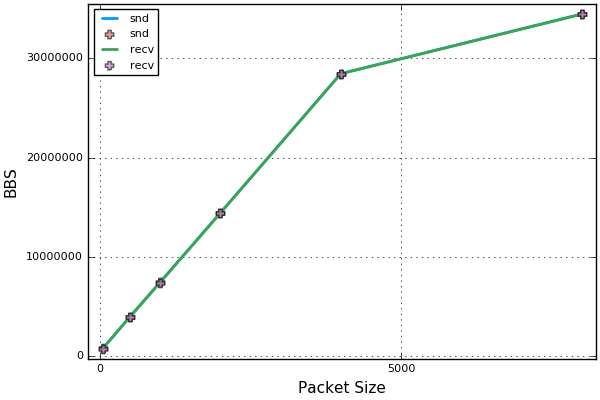
\includegraphics[scale=.6]{7.png}\\
\begin{center}
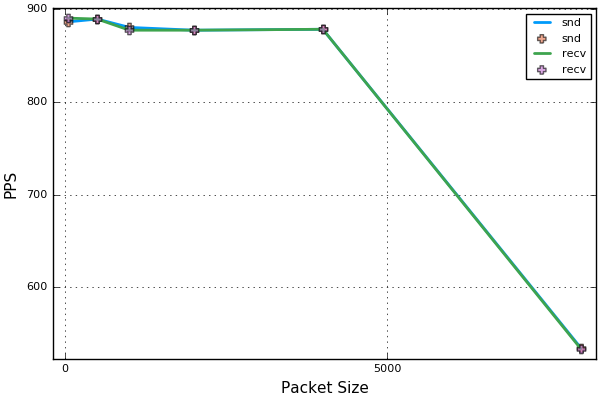
\includegraphics[scale=.6]{8.png}	
\end{center}
For small payload, the completion time and the PPS are consistent, and the throughput increases as payload increases. However, For payload size of $\geq$ 8000 bytes, we experience a slow down in completion time.
\end{problem}
\begin{problem}{3}
\end{problem}
\end{document}
